\chapter{Trasformata di Fourier}

\section{Nozioni preliminarie}

\subsection{Regressione lineare con il metodo dei minimi quadrati}
La regressione lineare \`e un'approssimazione di una serie di dati ad una
funzione lineare. Questa retta di approssimazione pu\`o essere calcolata in
molteplici modi, per questo progetto \`e di interesse utilizzare il
\emph{metodo dei minimi quadrati}.  Sar\`a dunque esplicato come trovare i
coefficienti di una retta a \(m+1\) termini interpolando \(N\) punti.
\begin{equation}
    r(x, a_0, \dots, a_m) = a_0 + x\sum_{i=1}^{m}a_i
\end{equation}
Consideriamo di avere gli insiemi \(X\) e \(Y\) entrambi con \(N\) termini di
cui si prende le coppie ordinate di valori, ossia i punti da interopolare.  Il
metodo dei minimi quadrati trova i coefficienti della retta minimizzando il
quadrato della differenza tra il valore stimato dalla retta \(y = r(x_k)\) e il
valore reale\(y_k\).
\begin{equation*}
    \min((r(x_k) - y_k)^2)\quad \forall x_k\in X,\, y_k\in Y
\end{equation*}
Definiamo quindi la funzione da minimizzare \(\varepsilon\)
\begin{equation}
    \varepsilon(a_0, \dots, a_m) = \sum_{k=1}^{N}\Big[r(x_k, a_0, \dots, a_m)  - y_k\Big]^2
\end{equation}
Da cui si computa le derivati parziali rispetto ai coefficienti ricercati,
ottenendo un sistema di equazioni lineare poich\`e si cerca per ogni derivata
quando essa equivale a 0. Ci\`o corrisponde anche ad affermare che il
\emph{gradiente} di \(\varepsilon\) \`e un vettore
\(\in\mathbb{R}^{m+1}\) con tutte le componenti a 0.
\begin{equation*}
    \nabla\varepsilon = (0, \dots, 0 )
\end{equation*}
A questo punto si pu\`o procedere risolvendo il sistema con l'algebra lineare
definendo la matrice di trasformazione \(\mathbf{A}\) e il vettore dei termini
noti \(\vec{u}\)
\begin{equation*}
    \nabla \varepsilon = \mathbf{A}
        \langle a_0, \dots,  a_m \rangle + \vec{u} \iff
    \langle a_0, \dots, a_m \rangle =
        \mathbf{A}^{-1}(-\vec{u})
\end{equation*}

\subsection{Funzione armonica}
Una funzione armonica, sinusoidale, pu\`o essere descritta in molteplici modi.
Iniziamo dunque osservando le forme pi\`u semplici, ossia la forma
trigonometrica.
\begin{align*}
    f(x) &= a\cdot\sin (\omega x + \varphi) \\
    f(x) &= b\cdot\cos(\omega x + \vartheta)
\end{align*}
Conoscendo la formula di Eulero 
\[
    e^{i\varphi} = \cos(\varphi) + i\cdot\sin(\varphi)
\]
possiamo riscrivere \(f(x)\) nei seguenti modi
\begin{align*}
    f(x) &= \frac{a}{2i}\cdot(e^{i(x\omega + \varphi)} - e^{-i(x\omega + \varphi)}) \\
    f(x) &= \frac{b}{2}\cdot(e^{i(x\omega + \vartheta)} + e^{-i(x\omega + \vartheta)})
\end{align*}

\subsection{Propriet\`a di ortogonalit\`a del seno e del coseno}
Per avere delle fondamenta solide prima dell'introduzione dell'argomento
principale, saranno dimostrate le propriet\`a di ortogonalit\`a del seno e
coseno. Considerando il periodo \(T\), dunque di frequenza \(2\pi /\,T\)
in uno spazio euclideo.

\subsubsection{Intuizione geometrica}

\begin{figure}[H] \centering
    \begin{tikzpicture}
        \begin{axis}[
            width = .5\textwidth,
            height = .5\textwidth,
            axis x line = center,
            axis y line = center,
            xlabel = {\(x\)},
            xlabel style = {right},
            ylabel = {\(y(x)\)},
            ylabel style = {above},
            grid=both,
            grid style = dotted,
            % axis equal,
            extra x ticks = {-10,-9,...,10},
            extra x tick labels= \empty,
            extra y ticks = {-10,-9,...,10},
            extra y tick labels= \empty,
            samples = 200,
            domain=0:2*pi,
            ymin=-1.25, ymax=1.25,
        ]
            \path[name path=axis] (axis cs:0,0) -- (axis cs: 2*pi,0);

            \addplot[red, name path=sin]{sin(deg(x))};
            \addplot[red, opacity=.1] fill between [
                of=sin and axis,
                soft clip={domain=0:2*pi}
            ];

            \addplot[blue, name path=cos]{cos(deg(x))};
            \addplot[blue, opacity=.1] fill between [
                of=cos and axis,
                soft clip={domain=0:2*pi}
            ];
        \end{axis}
    \end{tikzpicture}
    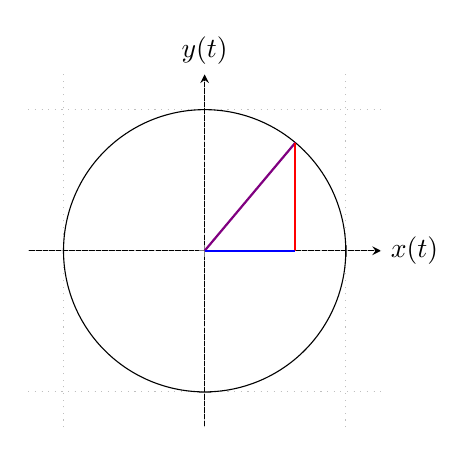
\begin{tikzpicture}[>=latex]
        \begin{axis}[
            width = .5\textwidth,
            height = .5\textwidth,
            axis x line = center,
            axis y line = center,
            xlabel = {\(x(t)\)},
            xlabel style = {right},
            ylabel = {\(y(t)\)},
            ylabel style = {above},
            grid=both,
            grid style = dotted,
            axis equal,
            xticklabels = \empty,
            yticklabels = \empty,
            extra x ticks = {-10,-9,...,10},
            extra x tick labels= \empty,
            extra y ticks = {-10,-9,...,10},
            extra y tick labels= \empty,
            xmin=-1.25, xmax=1.25,
            ymin=-1.25, ymax=1.25,
            samples=800,
        ]
            \addplot[mark=none,domain=0:360] ({cos(x)}, {sin(x)});

            \def\angle{50}
            \pgfmathsetmacro\ax{cos(\angle)}
            \pgfmathsetmacro\ay{sin(\angle)}

            \coordinate (a) at (\ax,\ay);
            \coordinate (o) at (0,0);
            \draw[thick, violet] (0,0) -- (a);
            \draw[thick, red] (a) -- (a |- o);
            \draw[thick, blue] (o) -- (a |- o);
        \end{axis}
    \end{tikzpicture}

    \caption{Funzioni \(\sin\) e \(\cos\) \label{fig:sin-cos-orth-plot}}
\end{figure}

Si pu\`o osservare intuitivamente dal cerchio unitario nella figura
\ref{fig:sin-cos-orth-plot} che le funzioni seno e coseno sono ortogonali tra
loro. Dal grafico a sinistra possiamo inoltre osservare che l'area (integrale)
di un periodo \`e sempre nulla.

\subsubsection{Dimostrzioni algebriche}
\begin{enumerate}
\item {
    Area di \(\sin\) in un periodo.
    \begin{align*}
        \int_0^T \sin(\frac{m2\pi x}{T})\,\dd{x} &= 0
        \quad \forall m \in \mathbb{Z} \\
        %
        \int_0^T \sin(\frac{m2\pi x}{T})\,\dd{x}
        &= \bigg [-\frac{T}{2\pi m }\cdot\cos\big(\frac{2\pi}{T}mx\big)\bigg]^T_0 \\
        &= -\frac{T}{2\pi m}\cdot\cos\big(2\pi m\big) 
            +\frac{T}{2\pi m}\cdot\cos\big(0\big) \\
        &= 0
    \end{align*}
}

\item {
    Area di \(\cos\) in un periodo.
    \begin{align*}
        \int_0^T \cos(\frac{m2\pi x}{T})\,\dd{x} &= 0
        \quad \forall m \in \mathbb{Z}^* \\
        %
        \int_0^T \cos(\frac{m2\pi x}{T})\,\dd{x}
        &= \bigg [\frac{T}{2\pi m}\cdot\sin\big(\frac{2\pi}{T}mx\big)\bigg]^T_0 \\
        &= \frac{T}{2\pi m}\cdot\sin\big(2\pi m\big) 
            +\frac{T}{2\pi m}\cdot\sin\big(0\big) \\
        &= \begin{cases}
            0 & \iff m \neq 0 \\
            T & \iff m = 0 
        \end{cases}
    \end{align*}
}

\item {
    Prodotto tra \(\sin\) e \(\cos\).
    \begin{align*}
        \int_0^T \sin(\frac{m2\pi x}{T})\cos(\frac{n2\pi x}{T})\,\dd{x} &= 0
        \quad \forall m,n \in \mathbb{Z} \\
        %
        \int_0^T \sin(\frac{m2\pi x}{T})\cos(\frac{n2\pi x}{T})\,\dd{x} &=
        \underbrace{\frac{1}{2}\int_0^T\sin\bigg[\frac{2\pi}{T}(n+m)x\bigg]\,\dd{x}}_{0} - 
        \underbrace{\frac{1}{2}\int_0^T\sin\bigg[\frac{2\pi}{T}(n-m)x\bigg]\,\dd{x}}_{0} \\
        %
        &= 0 \\
    \end{align*}
}

\item {
    Prodotto tra due \(\sin\) di frequenze diverse.
    \begin{align*}
        \int_0^T \sin(\frac{m2\pi x}{T})\sin(\frac{n2\pi x}{T})\,\dd{x} &= 0 
        \quad \forall m,n \in \mathbb{Z}~|~m\neq \pm n \\
        %
        \int_0^T \sin(\frac{m2\pi x}{T})\sin(\frac{n2\pi x}{T})\,\dd{x} &= 
        \underbrace{\frac{1}{2}\int_0^T\cos\bigg[\frac{2\pi}{T}(n-m)x\bigg]\,\dd{x}}_{m-n~\neq~0\implies 0} -
        \underbrace{\frac{1}{2}\int_0^T\cos\bigg[\frac{2\pi}{T}(n+m)x\bigg]\,\dd{x}}_{m+n~\neq~0\implies 0} \\
        %
        &= \begin{cases}
            0 & \iff n \neq \pm m \\
            T/2 & \iff n = m \\
            - T/2 & \iff n = - m \\
        \end{cases}
    \end{align*}
}

\item {
    Prodotto tra due \(\cos\) di frequenze diverse.
    \begin{align*}
        \int_0^T \cos(\frac{m2\pi x}{T})\cos(\frac{n2\pi x}{T})\,\dd{x} &= 0 
        \quad \forall m,n \in \mathbb{Z}^*~|~m\neq \pm n \\
        %
        \int_0^T \cos(\frac{m2\pi x}{T})\cos(\frac{n2\pi x}{T})\,\dd{x} &= 
        \underbrace{\frac{1}{2}\int_0^T\cos\bigg[\frac{2\pi}{T}(n+m)x\bigg]\,\dd{x}}_{m+n~\neq~0\implies 0} +
        \underbrace{\frac{1}{2}\int_0^T\cos\bigg[\frac{2\pi}{T}(n-m)x\bigg]\,\dd{x}}_{m-n~\neq~0\implies 0} \\
        %
        &= \begin{cases}
            0 & \iff n \neq \pm m \\
            T/2 & \iff n = \pm m \\
        \end{cases}
    \end{align*}
}

\item {
    \(\sin\) e \(\cos\) raggruppate nella forma complessa con la formula di Eulero.
    \begin{align*}
        \int_0^T e^{i2\pi kx/T}\,\dd{x} &= 0
        \quad \forall k \in \mathbb{Z}^* \\
        %
        \int_0^T e^{i2\pi kx/T}\,\dd{x} &=
        \underbrace{\int_0^T\cos(\frac{2\pi}{T} kx)\,\dd{x}}_{k\neq 0 \implies 0} + 
        \underbrace{i\int_0^T\sin(\frac{2\pi}{T} kx)\,\dd{x}}_{0}  \\
        %
        &= \begin{cases}
            0 & \iff k \neq 0 \\
            T & \iff k = 0
        \end{cases}
    \end{align*}
}
\end{enumerate}

% \begin{align*}
%     & \int_0^T \sin(\frac{m2\pi x}{T})\,\dd{x} = 0
%         \quad \forall m \in \mathbb{Z} \\
%     %
%     & \int_0^T \cos(\frac{m2\pi x}{T})\,\dd{x} = 0
%         \quad \forall m \in \mathbb{Z^*} \\
%     %
%     & \int_0^T \sin(\frac{m2\pi x}{T})\cos(\frac{n2\pi x}{T})\,\dd{x} = 0
%         \quad \forall m,n \in \mathbb{Z} \\
%     %
%     & \int_0^T \sin(\frac{m2\pi x}{T})\sin(\frac{n2\pi x}{T})\,\dd{x} = 0 
%         \quad \forall m,n \in \mathbb{Z}~|~m\neq \pm n \\
%     %
%     & \int_0^T \sin^2(\frac{m2\pi x}{T})\,\dd{x} = \frac{T}{2}
%         \quad \forall m \in \mathbb{Z} \\
%     %
%     & \int_0^T \cos(\frac{m2\pi x}{T})\cos(\frac{n2\pi x}{T})\,\dd{x} = 0 
%         \quad \forall m,n \in \mathbb{Z}~|~m\neq \pm n \\
%     %
%     & \int_0^T \cos^2(\frac{m2\pi x}{T})\,\dd{x} = \frac{T}{2}
%         \quad \forall m \in \mathbb{Z^*} \\
% \end{align*}

\section{Polinomio Trigonometrico}
Analogamente a come \`e definito un polinomio \(P\) ``normale'', una somma di
termini dal grado 0 fino al grado \(N\), \`e possibile definire anche un
polinomio trigonometrico \(T\).
\[
    P_N(x) = \sum_{n=0}^N a_n x^n \qquad a_n \in \mathbb{R},~ a_N \neq 0
\]
\[
    T_N(x) = \sum_{n=0}^N c_n e^{i\omega nx} 
        \qquad c_n \in\mathbb{C},~\omega\in\mathbb{R}, ~ c_N \neq 0
\]
Questo polinomio \`e detto \emph{trigonometrico} perch\`e utilizzando la
formula di eulero \(e^{i\varphi} = \cos(\varphi) + i\sin(\varphi)\) si pu\`o
espandere nel seguente modo.
\[
    T_N(x) = \sum_{n=0}^N\big [a_n\cdot\cos(\omega nx) + ib_n\cdot\sin(\omega nx)]
    \qquad a_n, b_n \in \mathbb{C}
\]
\`E definito inoltre il polinomio trogonometrico \emph{reale} come
\[
    T_N(x) = \sum_{n=0}^N\big [a_n\cdot\cos(\omega nx) + b_n\cdot\sin(\omega nx)]
    \qquad a_n, b_n \in \mathbb{R}
\]
Quest'ultimo mediante delle identit\`a trigonometriche pu\`o essere riscritto
anche nel modo seguente.
\[
    T_N(x) = \sum_{n=0}^N A_n\cdot\cos(\omega nx - \varphi)
\]

In tutti i casi possiamo osservare che il polinomio trogonometrico \`e una
somma di sinusoidi di frequenze multiple ad una base \(f = \omega/2\pi\).  Se
descritto mediante la terminologia dell'algebra lineare, si pu\`o anche
osservare che un polinomio trigonometrico \`e una combinazione lineare nello
spazio funzionale ortonormato dalle basi \(\sin(\omega x)\) e \(\cos(\omega
x)\).


\section{Serie di Fourier}

\section{Trasformata di Fourier discreta}
La Trasformata di Fouerier Discreta (DFT) \`e l'operazione matematica che
permette di trovare i coefficienti della serie di Fourier o di un polinomio
trigonometrico, per approssimare al meglio una funzione. Se presa a sestante
per\`o essa essendo una \emph{trasformata} pu\`o essere osservata anche come
una funzione che da uno spettro \emph{discreto} di una funzione. La densit\`a
spettrale ottenuta dalla DFT \`e dipende dalla frequenza di base scelta e nel
caso di un polinomio trigonometrico, anche dal numero di termini di
quest'ultimo.
\[
    \hat{f_k} = \frac{1}{T}\int_0^T f(x)\cdot e^{-ik2\pi fx}\,\dd{x}
\]

\subsection{Derivazione della DFT}
Per trovare la DFT, supponiamo di voler approssimare una funzione \(f\),
utilizzando il metodo dei minimi quadrati, con un polinomio trigonometrico
reale.
\[
    T_N(x) =  \sum_{n=0}^N A_n\cdot\cos(\omega nx -\varphi) \qquad \omega=2\pi f
\]
Sappiamo che questo pu\`o essere scritto anche nel seguente modo.
\[
    T_N(x) =  \sum_{n=0}^N a_n\cdot\cos(\omega nx)  + b_n\cdot\sin(\omega nx)
\]

Dunque per trovare i termini \(a_0,\dots,a_N\) e \(b_0,\dots,b_N\) definiamo
una funzione \(\varepsilon\) da minimizzare con il metodo dei minimi quadrati.
\[
    \varepsilon = \int_0^T\big[T_N(x) - f(x)\big]^2\,\dd{x}
\]

Per generalizzare sar\`a dimostrato come trovare il \(k\)-esimo termine.
\[
    \frac{\partial\varepsilon}{\partial a_k} =
    \frac{\partial}{\partial a_k} \int_0^T\big[T_N(x) - f(x)\big]^2\,\dd{x}
    = 0
\]
\[
    \frac{\partial\varepsilon}{\partial b_k} =
    \frac{\partial}{\partial b_k} \int_0^T\big[T_N(x) - f(x)\big]^2\,\dd{x}
    = 0
\]

\subsubsection{Termini dei coseni}
\begin{align*}
    \frac{\partial\varepsilon}{\partial a_k} =
    \frac{\partial}{\partial a_k} \int_0^T\big[T_N(x) - f(x)\big]^2\,\dd{x}
    &= 0 \\
\end{align*}
\subsubsection{Termini dei seni}

\section{Trasformata di Fourier}

\section{Interpretazione geometrica}

\section{Fast Fourier Transform}
\subsection{Motivazioni e Complessit\`a temporale}
\subsection{Propriet\`a dei numeri complessi}

% \section{}
